\chapter{dials buttons switches} 
\label{sec:dials}
\begin{definition}[Jeffrey Says\index{Jeffrey Says}]
\setlength{\intextsep}{0pt}%
\setlength{\columnsep}{3pt}%
\begin{wrapfigure}{l}{0.12\textwidth}

\includegraphics[width=\linewidth]{src/callout/psych.png} 
\end{wrapfigure}
\small
Gradually the idea solidified into the concept of a
light-show generator, something interactive, creative but simple
enough so that anyone could do it, yet complex enough to produce
breathtaking results once learned well. A program to do for light, in
fact, what a synthesiser does for sound.
\end{definition}

Dials, buttons, switches, and knobs that we can twiddle and adjust are at the heart of the 
Psychedelia player's experience. Fortunately they are mostly packaged up into presets and bursts,
as we have already seen. However it is possible, if you are prepared to clutch the game's manual
to your chest at night in bed, to configure many individual settings in all sorts of different ways.

In this penultimate chapter we'll take a look at the more interesting of these settings in some detail, develop
a better idea of how they are supposed to work, and figure out how they were incorporated into the core routines
we covereded in earlier chapters.

\begin{figure}[H]
    \centering
    \begin{adjustbox}{width=3cm,margin=11cm -12cm}
      
\includegraphics[width=12cm]{src/delay/delay-low.png}%
    \end{adjustbox}
    \begin{adjustbox}{width=10.5cm,center}
      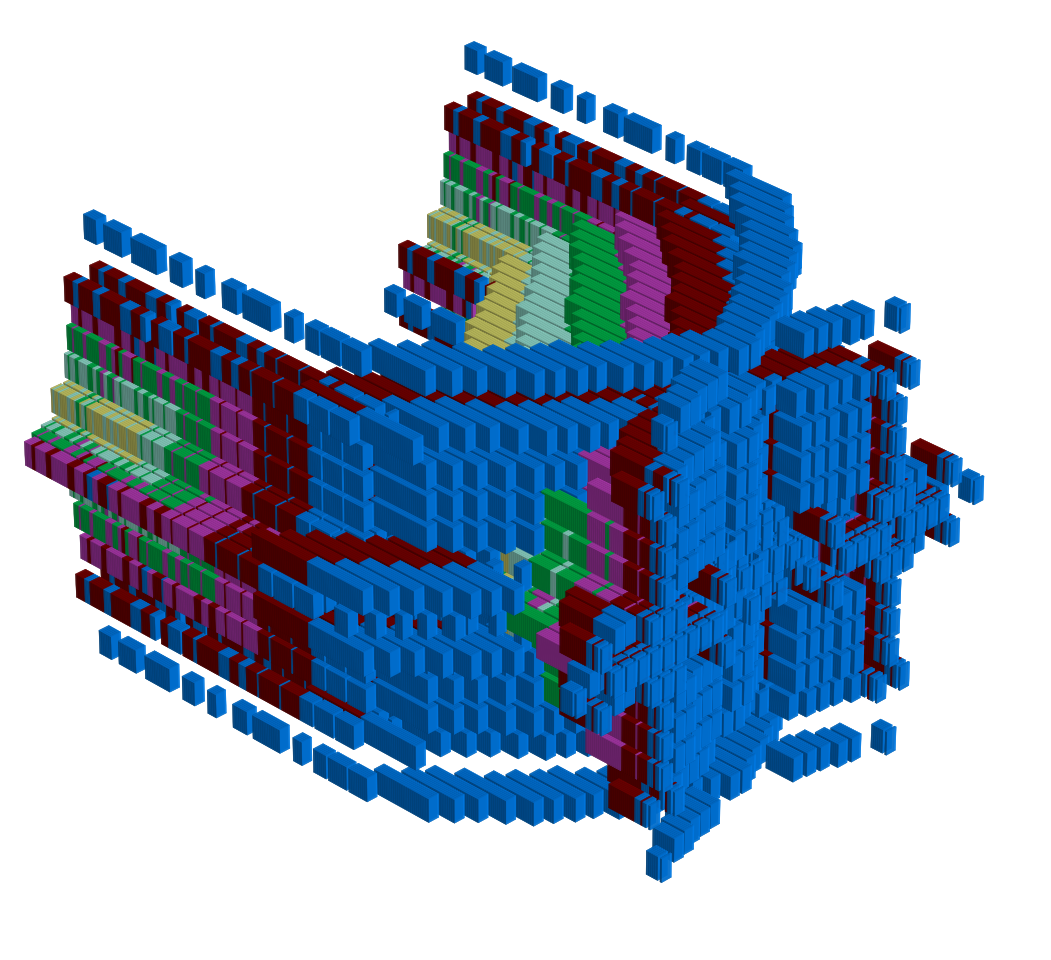
\includegraphics[width=12cm]{src/delay/pattern0-45.png}%
    \end{adjustbox}
    \begin{adjustbox}{width=3cm,margin=11cm -12cm}
      
\includegraphics[width=12cm]{src/delay/delay-high.png}%
    \end{adjustbox}
    \begin{adjustbox}{width=10.5cm,margin=0cm -2cm}
      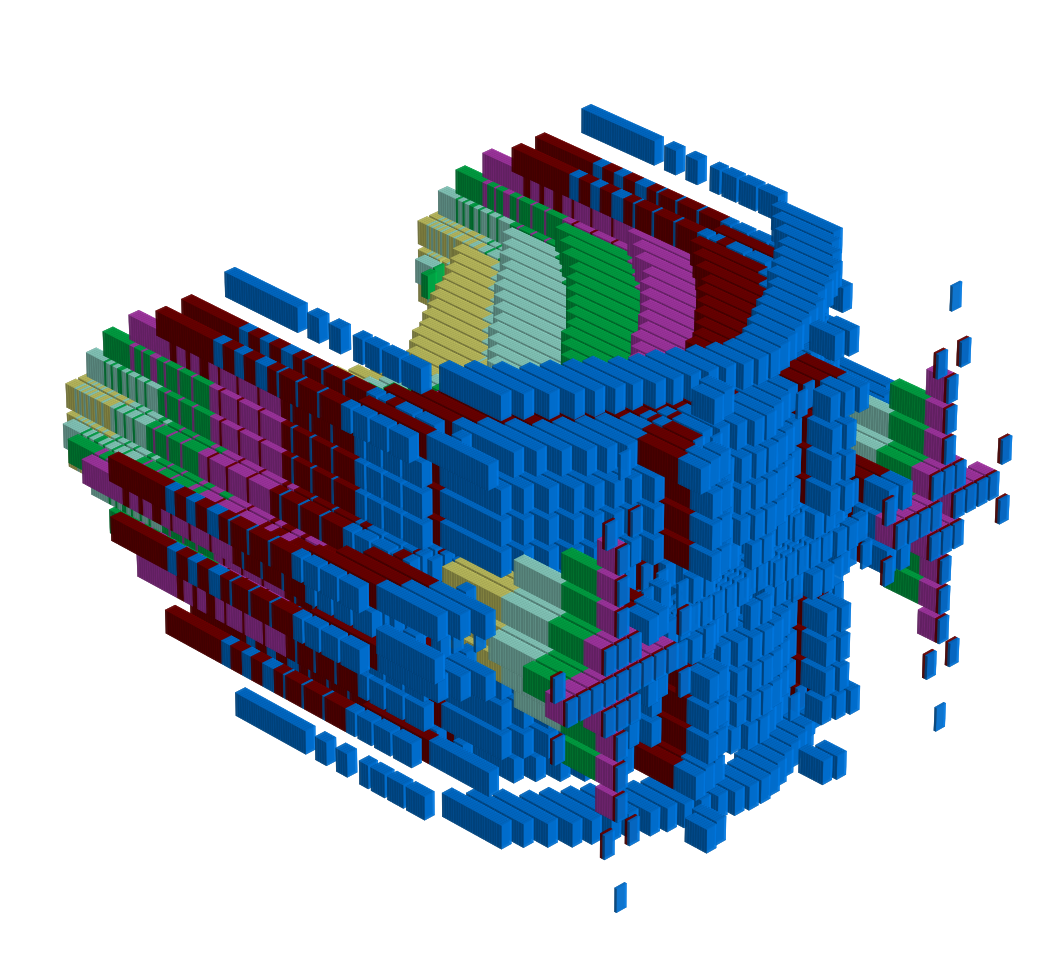
\includegraphics[width=12cm]{src/delay/pattern1-45.png}%
    \end{adjustbox}
    \caption{Effect of low and high values for Smoothing Delay}
\end{figure}
\clearpage

\section*{smoothing delay} 
\label{sec:delay}
\lstset{style=6502Style}
\lstset{ 
   aboveskip=5pt,
   belowskip=0pt,
}
Let's try to understand 'smoothing delay' better. Let's start by trying to understand
what it is. Perhaps Jeff Minter can shed some light:

\begin{definition}[Jeffrey Says\index{Jeffrey Says}]
\setlength{\intextsep}{0pt}%
\setlength{\columnsep}{3pt}%
\begin{wrapfigure}{l}{0.12\textwidth}

\includegraphics[width=\linewidth]{src/callout/psych.png} 
\end{wrapfigure}
\small
\textbf{D to activate:} Because of the time taken to
draw larger patterns speed increase/decrease is not linear. You
can adjust the ‘compensating delay’ which often smooths out jerky
patterns. Can be used just for special FX, though. Suck it and see.
\end{definition}

So that's clear then. Smoothing delay is what you want to use when
you need to smooth out the delay. What more explanation could we need?

If we look at the effect of setting this parameter to its lowest and
highest possible value opposite, the difference in behaviour is not
extreme. It's almost quite subtle. With a higher setting the pattern
evolves in a more drawn out fashion - as though a higher value lets
Psychedelia linger a little longer on the current state of the pattern
rather than immediately evolving it to the next state.

Let's dig into the code and see if this intuition is correct.

First of all though we'll take a look at the code that allows us to
twiddle this:

    \begin{adjustbox}{width=9cm}
      \frame{
\includegraphics[width=12cm]{src/delay/delay-low.png}}%
    \end{adjustbox}

to this:

    \begin{adjustbox}{width=8.2cm}
      \frame{
\includegraphics[width=12cm]{src/delay/delay-high.png}}%
    \end{adjustbox}

\clearpage

\textbf{Lines 1297-1303. \icode{\textbf{MaybeDPressed}}}
\begin{lstlisting}[caption=From \icode{CheckKeyboardInput\index{CheckKeyboardInput}}.,escapechar=\%]
MaybeDPressed   
        CMP #KEY_D ; 'D' pressed?
        BNE MaybeCPressed

DPressed
        LDA #$01
        STA currentVariableMode%\index{currentVariableMode}%
        RTS 
\end{lstlisting}
\textbf{Lines 1838-1868. \icode{\textbf{UpdateVariableDisplay}}}
\begin{lstlisting}[caption=From \icode{CheckKeyboardInputForActiveVariable}.,escapechar=\%]
UpdateVariableDisplay   
        ...

        LDX currentVariableMode%\index{currentVariableMode}%
        LDA lastKeyPressed%\index{lastKeyPressed}%
        CMP #KEY_GT ; > pressed?
        BNE MaybeLeftArrowPressed

RightArrowPressed
        ; > pressed, increase the value bar.
        INC presetValueArray%\index{presetValueArray}%,X
        LDA presetValueArray%\index{presetValueArray}%,X
        ; Make sure we don't exceed the max value.
        CMP maxValueForPresetValueArray,X
        BNE MaybeInColorMode%\index{MaybeInColorMode}%
        DEC presetValueArray%\index{presetValueArray}%,X
        JMP MaybeInColorMode%\index{MaybeInColorMode}%

MaybeLeftArrowPressed   
        CMP #KEY_LT ; < pressed?
        BNE MaybeInColorMode%\index{MaybeInColorMode}%

        ; < pressed, decrease the value bar.
        DEC presetValueArray%\index{presetValueArray}%,X
        LDA presetValueArray%\index{presetValueArray}%,X
        ; Make sure we don't exceed the min value.
        CMP minValueForPresetValueArray,X
        BNE MaybeInColorMode%\index{MaybeInColorMode}%
        INC presetValueArray%\index{presetValueArray}%,X

\end{lstlisting}
\clearpage
\rhead[]{\icode{MaybeDPressed, UpdateVariableDisplay}}
\textbf{Lines 1297-1303. \icode{\textbf{MaybeDPressed}}:} When \icode{D} is pressed we don't
update a setting there and then as you might expect. Instead we get ready to display the 'Smoothing
Delay' control bar, by... loading the value \icode{\$01} to \icode{currentVariableMode\index{currentVariableMode}}? Okay, we'll
go with that for now.

\textbf{Lines 1838-1868. \icode{\textbf{UpdateVariableDisplay}}:}  The next time we loop around
to \icode{Check\-KeyboardInput}, we hit this little piece of logic at the very top of it:

\begin{lstlisting}[escapechar=\%]
CheckKeyboardInput%\index{CheckKeyboardInput}%   
        LDA currentVariableMode%\index{currentVariableMode}%
        BEQ CheckForGeneralKeystrokes
        JMP CheckKeyboardInputForActiveVariable
\end{lstlisting}

Well, we just loaded \icode{\$01} to \icode{currentVariableMode\index{currentVariableMode}} above so it's not zero.  It follows that
the \icode{BEQ} check will give a negative result (the check means 'is the value in \icode{A} equal to zero?'), 
so instead of forking to \icode{CheckForGeneralKeystrokes} we'll \icode{JMP} to \icode{CheckKeyboardInputForActiveVariable}.

This is where the function we're looking at here lives. As we can see the first thing it does is load 
\icode{currentVariableMode\index{currentVariableMode}} to the \icode{X} register. This is because we're going to use it as an index
into an array we encountered in the previous chapter on Presets. This is the array \icode{presetValueArray\index{presetValueArray}}
which contains a lot of the settings we'll be looking at in this chapter huddled together like a gaggle
of ducklings, with \icode{smoothingDelay\index{smoothingDelay}} near the head at index 1 (index 0 being taken by \icode{unusedPresetByte}):

\begin{lstlisting}[escapechar=\%]
presetValueArray%\index{presetValueArray}%
unusedPresetByte        .BYTE $00
smoothingDelay%\index{smoothingDelay}%          .BYTE $0C
cursorSpeed             .BYTE $02
bufferLength%\index{bufferLength}%            .BYTE $1F
pulseSpeed              .BYTE $01
...
\end{lstlisting}

With \icode{X} set to 1 we can now use it increment the value for \icode{smoothingDelay\index{smoothingDelay}} by
simply executing:
\begin{lstlisting}[escapechar=\%]
        INC presetValueArray%\index{presetValueArray}%,X
\end{lstlisting}
And decrement it by doing:
\begin{lstlisting}[escapechar=\%]
        DEC presetValueArray%\index{presetValueArray}%,X
\end{lstlisting}
This is handy, and worth remembering as the technique will be reused for adjusting other values that 
we look at that also live in \icode{presetValueArray\index{presetValueArray}}.

\clearpage

\textbf{Lines 923-928. \icode{\textbf{ApplySmoothingDelay}}}
\begin{lstlisting}[caption=From \icode{MainInterruptHandler}.,escapechar=\%]
ApplySmoothingDelay    
        LDA smoothingDelay%\index{smoothingDelay}%
        STA initialSmoothingDelayForStep,X
        STA smoothingDelayForStep,X
\end{lstlisting}
\textbf{Lines 644-679. \icode{\textbf{ShouldDoAPaint}}}
\begin{lstlisting}[caption=From \icode{MainPaintLoop\index{MainPaintLoop}}.,escapechar=\%]
ShouldDoAPaint   
        ...
        DEC smoothingDelayForStep,X
        BNE GoBackToStartOfLoop

        ; Actually paint some pixels to the screen.
        ; Reset the delay for this step.
        LDA initialSmoothingDelayForStep,X
        STA smoothingDelayForStep,X

        ; Get the x and y positions for this pixel.
        LDA pixelXPositionArray%\index{pixelXPositionArray}%,X
        STA pixelXPositionZP
        LDA pixelYPositionArray%\index{pixelYPositionArray}%,X
        STA pixelYPositionZP

        LDA patternIndexArray%\index{patternIndexArray}%,X
        STA presetIndex

        LDA symmetrySettingForStepCount%\index{symmetrySettingForStepCount}%,X
        STA currentSymmetrySettingForStep%\index{currentSymmetrySettingForStep}%

        LDA currentIndexToColorValues
        AND #$80
        BNE ResetAndGoBackToStartOfLoop

        TXA 
        PHA 
        JSR PaintStructureAtCurrentPosition
        PLA 
        TAX 
\end{lstlisting}
\clearpage

\rhead[]{\icode{ApplySmoothingDelay, ShouldDoAPaint}}
\textbf{Lines 923-928. \icode{\textbf{ApplySmoothingDelay}}:} With the player's selected value loaded 
safely to \icode{smoothingDelay\index{smoothingDelay}} we now have to see how it is applied to the evolution of the patterns.

The immediate answer to this is given here: it is loaded to the current position in the 
\icode{smoothingDelayForStep} and \icode{initialSmoothingDelayForStep} arrays. Remember that these
arrays, along with several others, help track the different phases in the evolution of the pattern.


\textbf{Lines 644-679. \icode{\textbf{ShouldDoAPaint}}:}  Back to the main paint loop, where the
pixel painting is actually done. We looked at this loop in detail in earlier chapters. And it is in
here that we see the 'smoothing delay' get applied. At the top of function we've extracted here
the value in \icode{smoothingDelayForStep} is used as a countdown counter. This is what our
smoothing delay is: a counter that we decrement at each pass. If it's not zero yet (\icode{BNE}),
we \icode{GoBackToStartOfLoop}.

If it is zero we can actually paint a pixel. We use the value in \icode{initialSmoothing\-DelayForStep}
to reset our counter and get on with doing a full paint.

So after all that we can see that 'smoothing delay' acts as a brake on the painting loop - the greater
the value the longer it will defer the next paint, resulting in a slower and smoother evolution of the
pattern being painted.

\begin{figure}[H]
    \centering
    \begin{adjustbox}{width=10.5cm,center}
      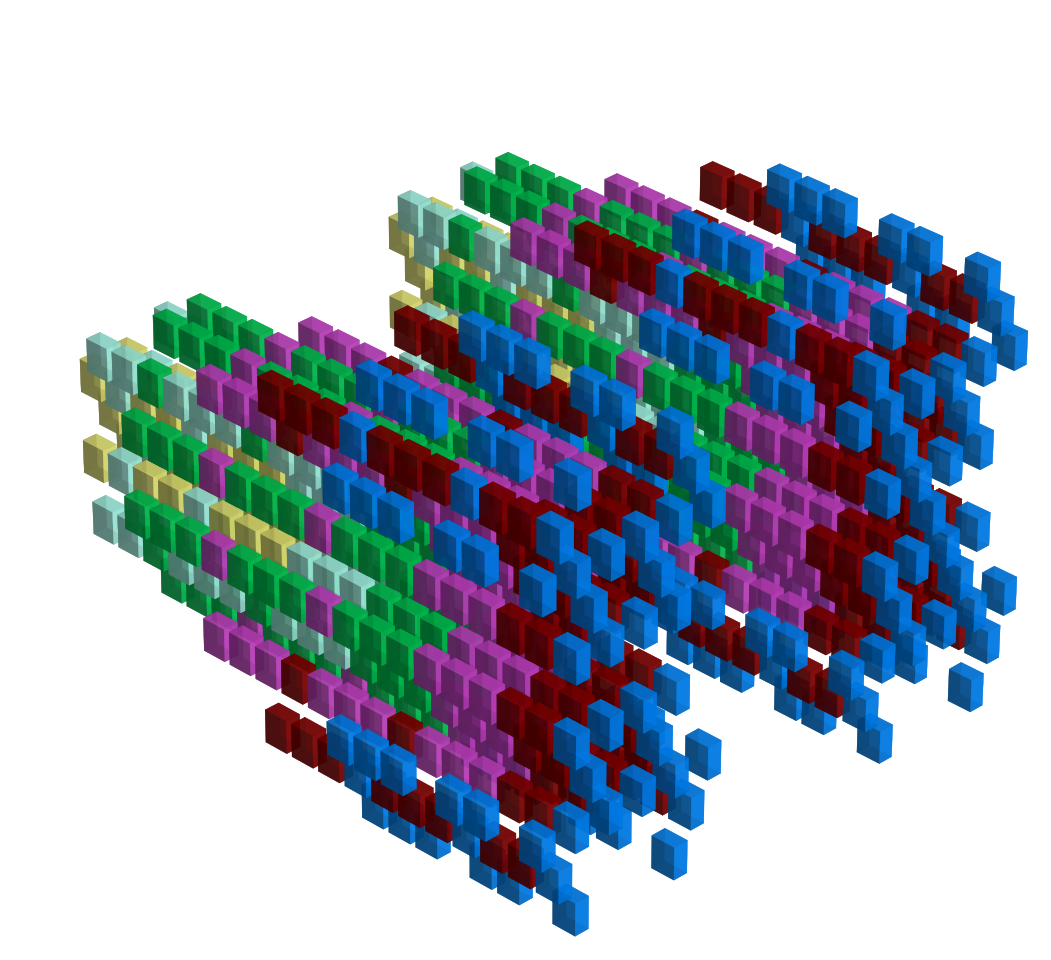
\includegraphics[width=12cm]{src/tracking/pattern1-0-45.png}%
    \end{adjustbox}
    \begin{adjustbox}{width=10.5cm,margin=0cm -2cm}
      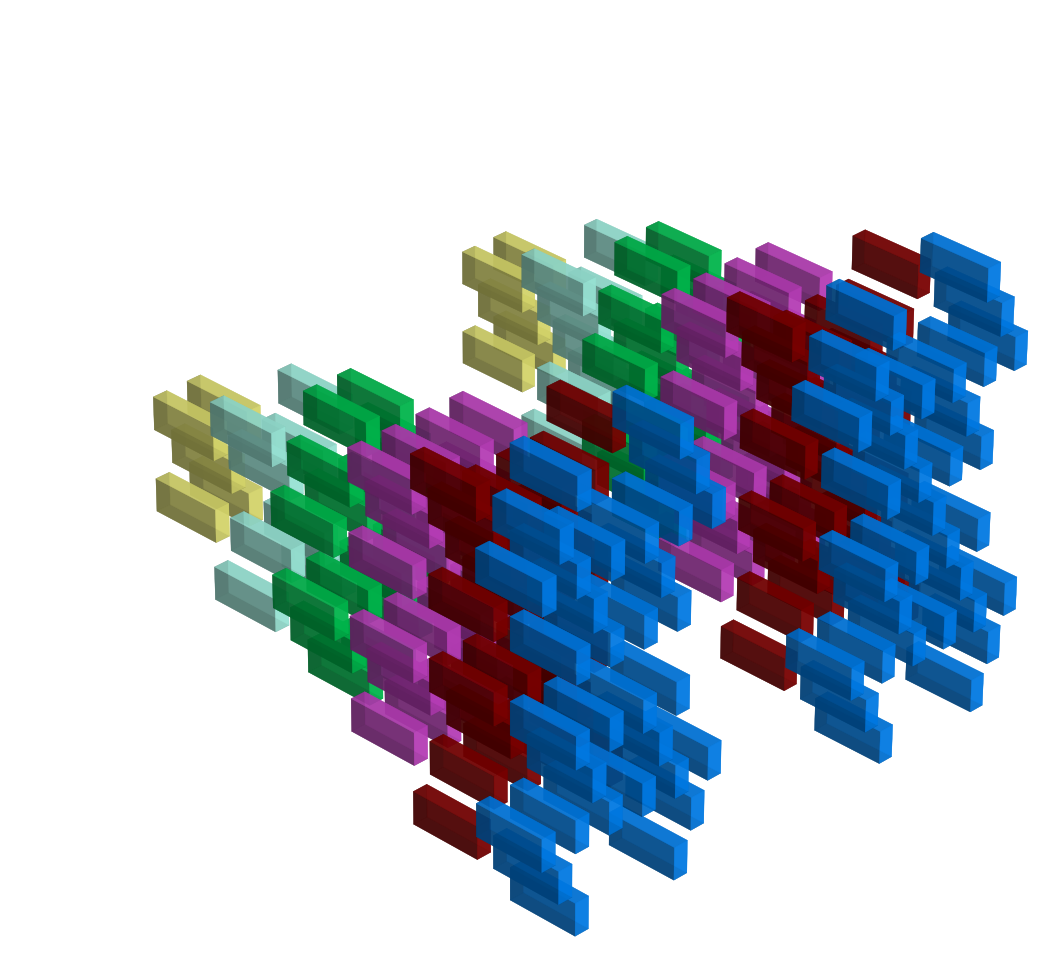
\includegraphics[width=12cm]{src/tracking/pattern1-1-45.png}%
    \end{adjustbox}
    \caption{Tracking 'on' (top) and 'off' (bottom).}
\end{figure}
\clearpage

\rhead[]{tentative tracking}
\section*{tentative tracking} 
\label{sec:tracking}
\lstset{style=6502Style}
\lstset{ 
   aboveskip=5pt,
   belowskip=0pt,
}

\begin{definition}[Jeffrey Says\index{Jeffrey Says}]
\setlength{\intextsep}{0pt}%
\setlength{\columnsep}{3pt}%
\begin{wrapfigure}{l}{0.12\textwidth}

\includegraphics[width=\linewidth]{src/callout/psych.png} 
\end{wrapfigure}
\small
\textbf{T to Activate:} Controls\index{Controls} whether logic-seeking is used in
the buffer or not. The upshot of this for you is a slightly different
feel - continuous but fragmented when ON, or together-ish bursts
when OFF. Try it.
\\
\end{definition}

Tracking is 'on' by default and nearly all off the figures and diagrams we've used to illustrate
Psychedelia's behaviour have demonstrated the behaviour of 'tracking'. In essence, tracking means
using the values previously painted to a pixel position on screen as partial feedback into the next
color value that we will paint into it. 

When tracking is enabled the colors of pixels will change much more often, whereas when it is disabled
the display becomes much less interesting, with a more consistent and smoother evolution in the colors
of the patterns as they evolve.

\clearpage
\textbf{Lines 1362-1390. \icode{\textbf{MaybeTPressed\index{MaybeTPressed}}}} 
\begin{lstlisting}[escapechar=\%]
;-------------------------------------------------------
; CheckKeyboardInput%\index{CheckKeyboardInput}%
;-------------------------------------------------------
CheckKeyboardInput%\index{CheckKeyboardInput}%   
    ...
MaybeTPressed   
    CMP #KEY_T ; T pressed.
    BNE CheckIfPresetKeysPressed

    ; Toggle tracking on or off.
    LDA trackingActivated%\index{trackingActivated}%
    EOR #$FF
    STA trackingActivated%\index{trackingActivated}%

    ; Use the new setting to get an offset into our screen message.
    ; in txtTrackingOnOff
    AND #$01
    ASL 
    ASL 
    ASL 
    ASL 
    TAY 

    JSR ClearLastLineOfScreen%\index{ClearLastLineOfScreen}%

    ; Display the updated setting of 'tracking'.
    LDX #$00
txtTrackingLoop   
    LDA txtTrackingOnOff,Y
    STA lastLineBufferPtr,X
    INY 
    INX 
    CPX #$10
    BNE txtTrackingLoop

    JMP WriteLastLineBufferToScreen%\index{WriteLastLineBufferToScreen}%
    RTS 
\end{lstlisting}
\clearpage
\rhead[]{\icode{MaybeTPressed}}
\textbf{Lines 1362-1390. \icode{\textbf{MaybeTPressed}}:} 
Pressing \icode{T} toggles tracking on or off. Tracking's on/off state is 
stored in \icode{trackingActivated\index{trackingActivated}}, with \icode{\$00} meaning 'off' and
\icode{\$FF} meaning 'on'. This means we can use a neat, economical trick
for toggling the value every time the user presses the 'T' key:

\begin{lstlisting}[escapechar=\%]
    ; Toggle tracking on or off.
    LDA trackingActivated%\index{trackingActivated}%
    EOR #$FF
    STA trackingActivated%\index{trackingActivated}%
\end{lstlisting}

The \icode{EOR} statement performs an exclusive-or that has the neat property of
turning \icode{\$00} into \icode{\$FF} and \icode{\$FF} into \icode{\$00} - equivelent
to switching a value on or off.

This is what the the bit by bit operation looks like when '\icode{EOR \$FF}' turns
\icode{trackingActivated\index{trackingActivated}} 'on':

\begin{figure}[H]
  {
    \setlength{\tabcolsep}{3.0pt}
    \setlength\cmidrulewidth{\heavyrulewidth} % Make cmidrule = 
    \begin{adjustbox}{width=7cm,center}

      \begin{tabular}{rllllllll}
        \toprule
        Byte & Bit 7 & Bit 6 & Bit 5 & Bit 4 & Bit 3 & Bit 2 & Bit 1 & Bit 0        \\
        \midrule
        \$00 & 0 & 0 & 0 & 0 & 0 & 0 & 0 & 0 \\
        \$FF & 1 & 1 & 1 & 1 & 1 & 1 & 1 & 1 \\
        \midrule
        Result & 1 & 1 & 1 & 1 & 1 & 1 & 1 & 1 \\
        \addlinespace
        \bottomrule
      \end{tabular}

    \end{adjustbox}

  }\caption*{X-OR'ing \$FF and \$00 gives \$FF, the 'on' value for \icode{trackingActivated\index{trackingActivated}}.}
\end{figure}

And this is what it looks like when \icode{EOR \$FF} turns \icode{trackingActivated\index{trackingActivated}} 'off' again:
\begin{figure}[H]
  {
    \setlength{\tabcolsep}{3.0pt}
    \setlength\cmidrulewidth{\heavyrulewidth} % Make cmidrule = 
    \begin{adjustbox}{width=7cm,center}

      \begin{tabular}{rllllllll}
        \toprule
        Byte & Bit 7 & Bit 6 & Bit 5 & Bit 4 & Bit 3 & Bit 2 & Bit 1 & Bit 0        \\
        \midrule
        \$FF & 1 & 1 & 1 & 1 & 1 & 1 & 1 & 1 \\
        \$FF & 1 & 1 & 1 & 1 & 1 & 1 & 1 & 1 \\
        \midrule
        Result & 0 & 0 & 0 & 0 & 0 & 0 & 0 & 0 \\
        \addlinespace
        \bottomrule
      \end{tabular}

    \end{adjustbox}

  }\caption*{X-OR'ing \$FF and \$FF gives \$00, the 'off' value for \icode{trackingActivated\index{trackingActivated}}.}
\end{figure}
\clearpage

\clearpage
\textbf{Lines 728-943. \icode{\textbf{MainInterruptHandler}}} 
\begin{lstlisting}[escapechar=\%]
;-------------------------------------------------------
; MainInterruptHandler
;-------------------------------------------------------
MainInterruptHandler
        ...
        ; Finally, update the pixel buffers with a byte
        ; each for the current pattern.        
UpdatePixelBuffersForPattern    
        INC currentStepCount%\index{currentStepCount}%
        LDA currentStepCount%\index{currentStepCount}%
        CMP bufferLength%\index{bufferLength}%
        BNE UpdateBaseLevelArray

        LDA #$00
        STA currentStepCount%\index{currentStepCount}%

UpdateBaseLevelArray   
        TAX 
        LDA currentColorIndexArray%\index{currentColorIndexArray}%,X
        CMP #$FF
        BEQ UpdatePositionArrays

CheckIfTrackingActivated
        LDA previousIndexToPixelBuffers%\index{previousIndexToPixelBuffers}%
        AND trackingActivated%\index{trackingActivated}%
        BEQ DrawCursorAndReturnFromInterrupt%\index{DrawCursorAndReturnFromInterrupt}%

        TAX 
        LDA currentColorIndexArray%\index{currentColorIndexArray}%,X
        CMP #$FF
        BNE DrawCursorAndReturnFromInterrupt%\index{DrawCursorAndReturnFromInterrupt}%

        STX currentStepCount%\index{currentStepCount}%

UpdatePositionArrays   
        LDA cursorXPosition%\index{cursorXPosition}%
        STA pixelXPositionArray%\index{pixelXPositionArray}%,X
        LDA cursorYPosition%\index{cursorYPosition}%
        STA pixelYPositionArray%\index{pixelYPositionArray}%,X

        ...
DrawCursorAndReturnFromInterrupt%\index{DrawCursorAndReturnFromInterrupt}%    
        LDA #$01
        STA currentColorToPaint%\index{currentColorToPaint}%
        JSR PaintCursorAtCurrentPosition%\index{PaintCursorAtCurrentPosition}%
        ; Falls through
\end{lstlisting}
\clearpage

\rhead[]{\icode{MainInterruptHandler}}
\textbf{Lines 728-943. \icode{\textbf{MainInterruptHandler}}:} 
As you may remember the \icode{MainInterruptHandler} runs every 1/60th of a
second.  You may also recall its main job is to fill the pixel buffers (e.g.
pixelXPositionArray\index{pixelXPositionArray}, pixelYPositionArray\index{pixelYPositionArray} and so on) so that the MainPaintLoop\index{MainPaintLoop}
can use them to paint the screen. 

\textbf{Lines 890-896. \icode{\textbf{CheckIfTrackingActivated}}:} 
\icode{trackingActivated\index{trackingActivated}} comes into play here. The idea is that if 'tracking'
is enabled then we should do a re-paint of the last entry in the buffers that was
processed by \icode{MainPaintLoop\index{MainPaintLoop}}. Naturally, if a pixel is being painted twice
over this will create a 'tracking' effect, as though the pattern is trailing a 
glowing tail after it.

We use the value in \icode{trackingActivated\index{trackingActivated}} to decide whether or not to paint
the previously processed position in the buffers by simply \icode{AND}'ing the
two together.

\begin{lstlisting}[escapechar=\%]
        LDA previousIndexToPixelBuffers%\index{previousIndexToPixelBuffers}%
        AND trackingActivated%\index{trackingActivated}%
        BEQ DrawCursorAndReturnFromInterrupt%\index{DrawCursorAndReturnFromInterrupt}%
\end{lstlisting}

If it's zero, we bail out
completely until the next interrupt by jumping to \icode{DrawCursor\-AndReturnFromInterrupt}.
But if we get a non-zero value that means tracking is enabled and 
we should go ahead and refresh the values in the buffers at the index given
by the value in \icode{previousIndex\-ToPixelBuffers}. So we 'fall through' instead to
\icode{UpdatePositionArrays} and a number of other sub-routines that update the
values of the previous position in our pixel buffers.

\clearpage
\begin{figure}[H]
    \centering
    \begin{adjustbox}{width=15cm,center}
      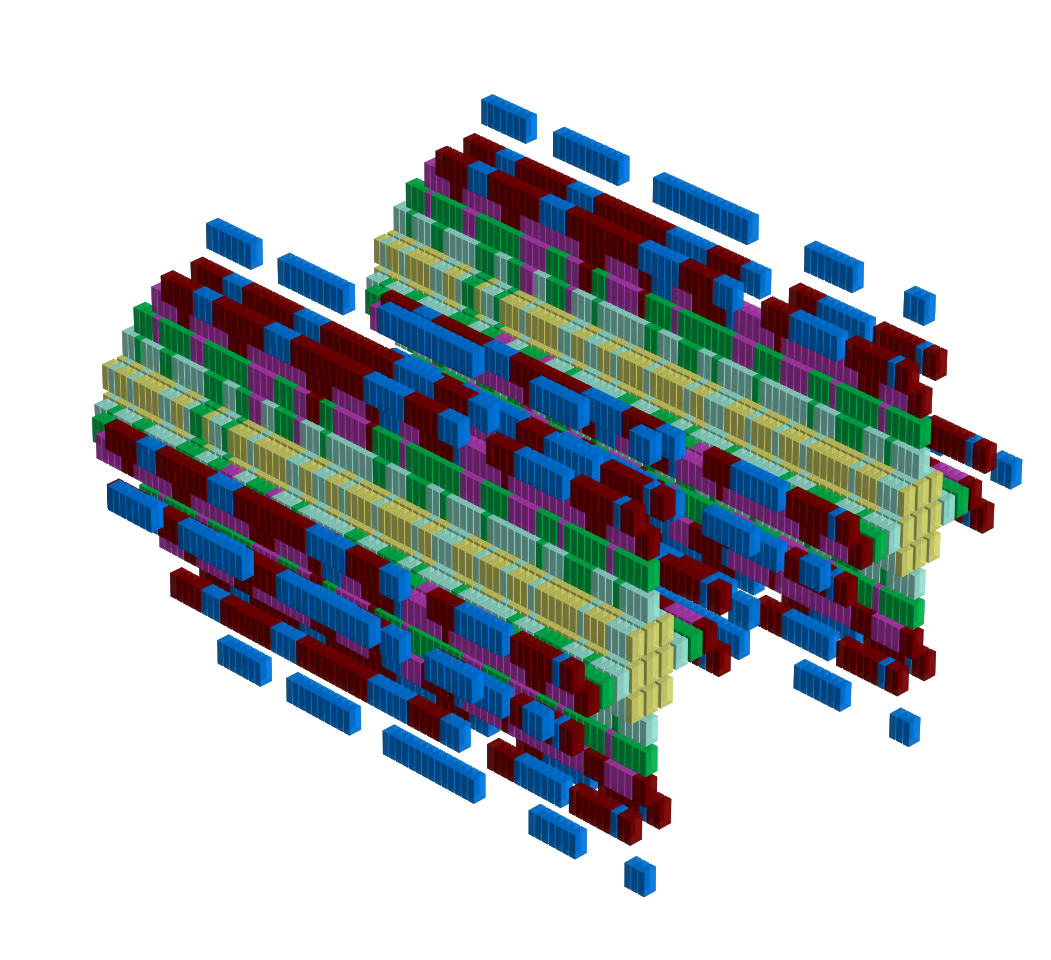
\includegraphics[width=10cm]{src/pulsespeed/pattern0-45.png}%
      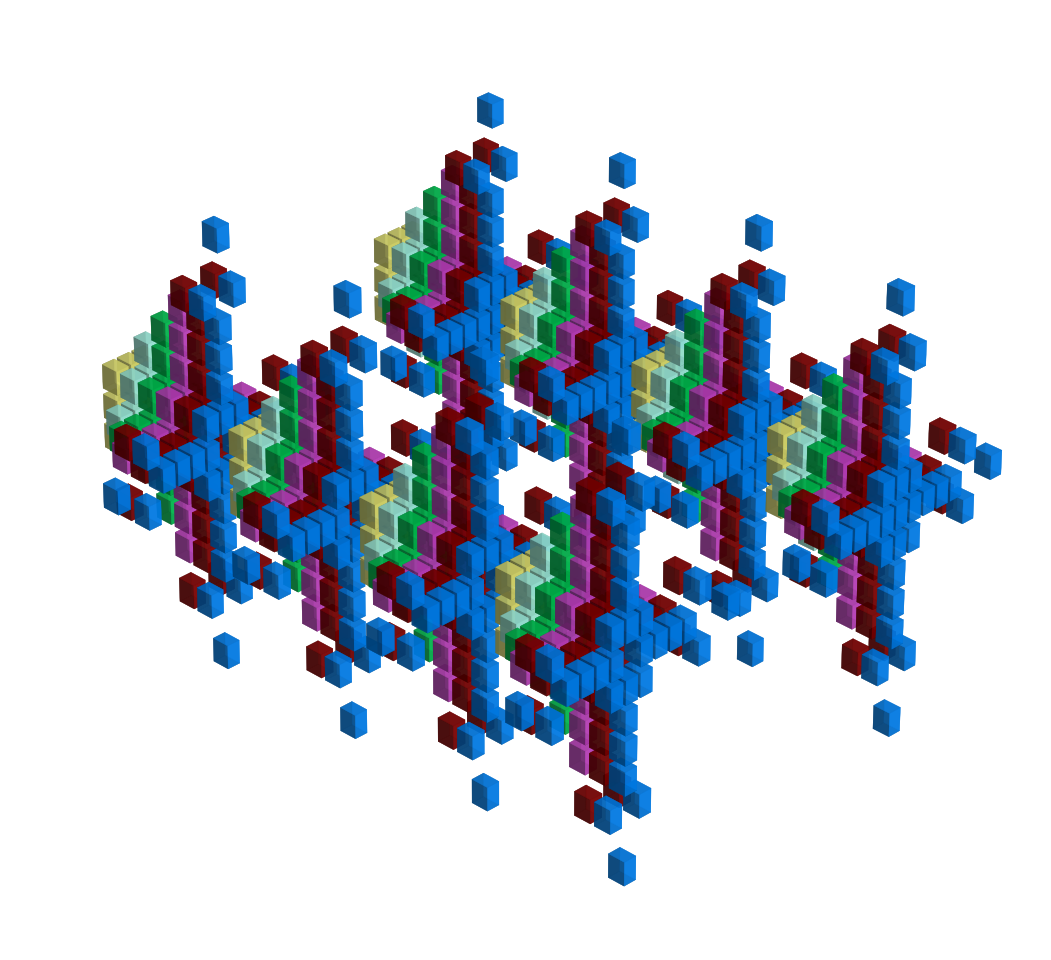
\includegraphics[width=10cm]{src/pulsespeed/pattern1-45.png}%
    \end{adjustbox}
    \caption{Effect of low and high values for Pulse Speed}
\end{figure}
\begin{figure}[H]
    \centering
    \begin{adjustbox}{width=15cm,center}
      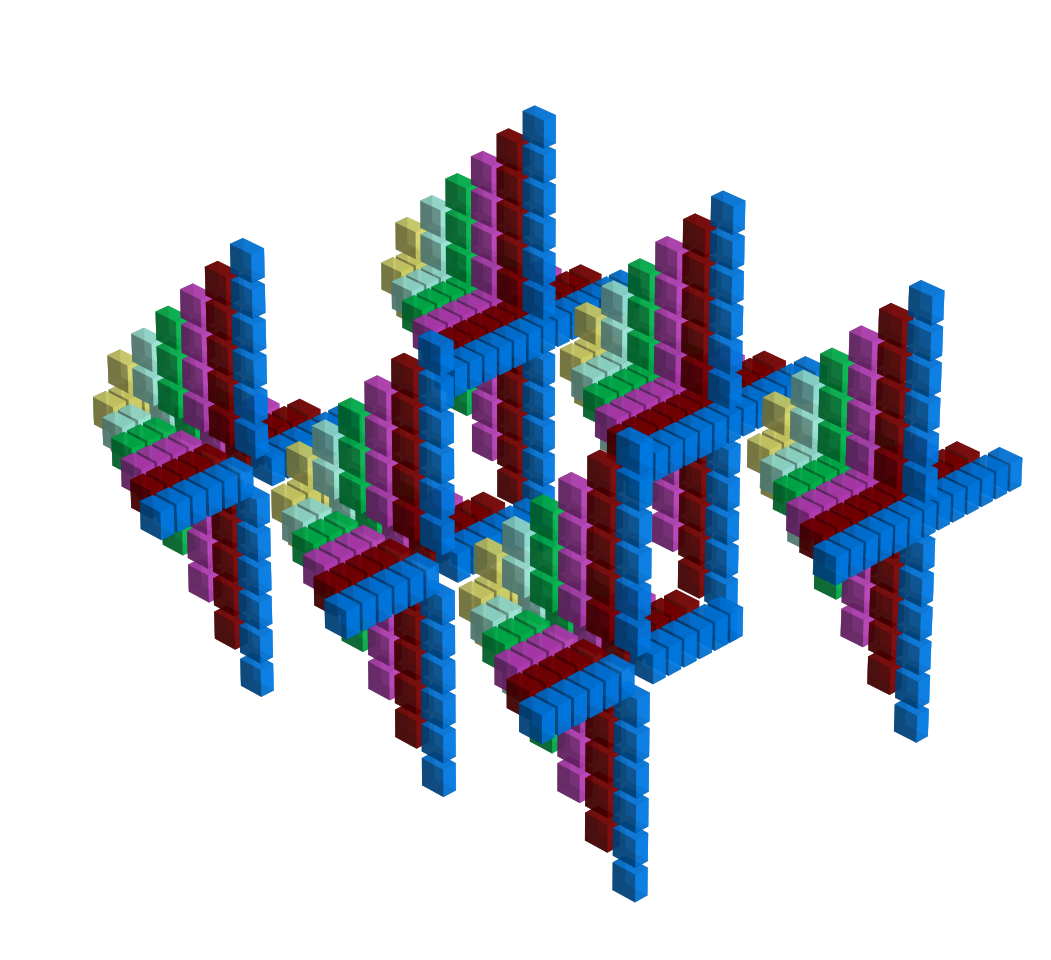
\includegraphics[width=10cm]{src/pulsewidth/pattern0-45.png}%
      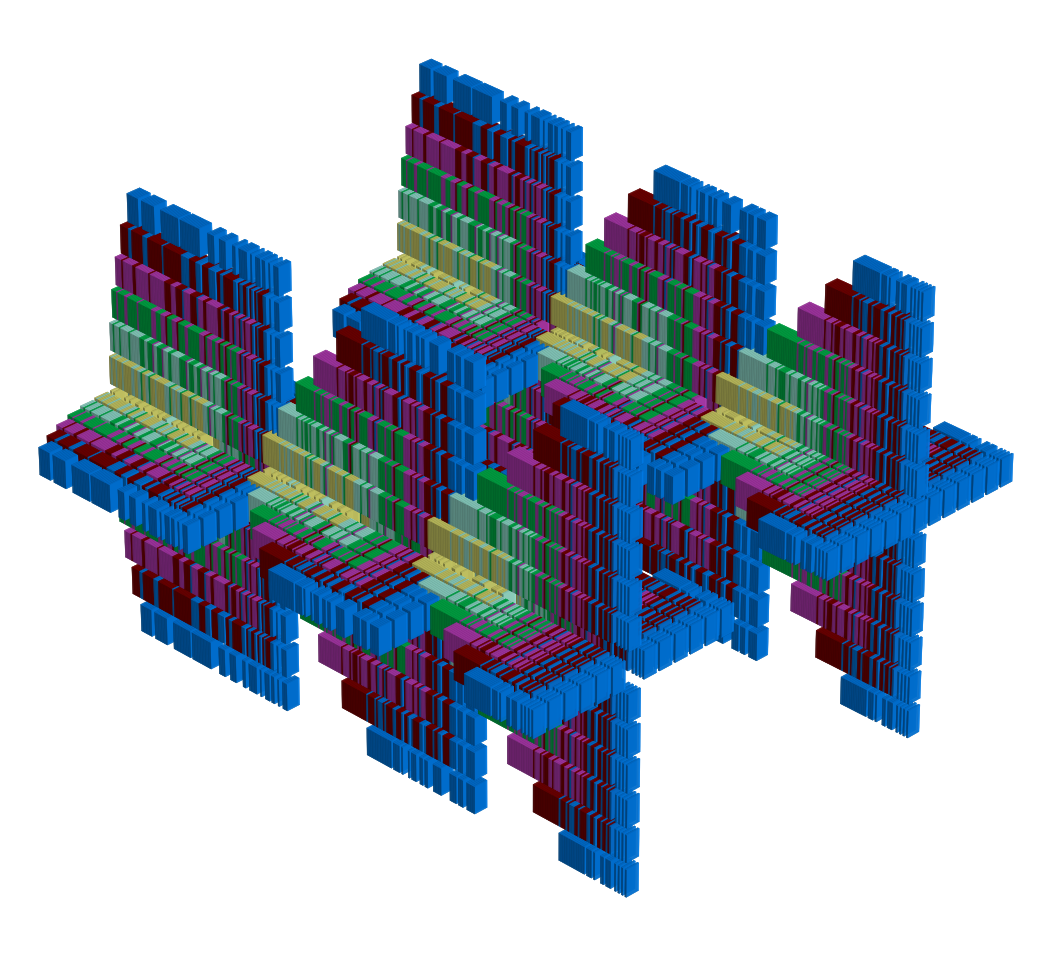
\includegraphics[width=10cm]{src/pulsewidth/pattern1-45.png}%
    \end{adjustbox}
    \caption{Effect of low and high values for Pulse Width}
\end{figure}
\clearpage
\rhead[]{pulse speed, pulse width}
\section*{pulse speed}
\label{sec:pulse_speed}
\lstset{style=6502Style}
\lstset{ 
   aboveskip=5pt,
   belowskip=0pt,
}

\begin{definition}[Jeffrey Says\index{Jeffrey Says}]
\setlength{\intextsep}{0pt}%
\setlength{\columnsep}{3pt}%
\begin{wrapfigure}{l}{0.12\textwidth}

\includegraphics[width=\linewidth]{src/callout/psych.png} 
\end{wrapfigure}
\small
\textbf{P to activate:} Usually if you hold down the button
you get a continuous stream. Setting the Pulse Speed allows you to
generate a pulsed stream, as if you were rapidly pressing and
releasing the FIRE button.
\\
\end{definition}

Pulsing is self explanatory enough, especially when you compare the
illustrations opposite. In a way, pulse width behaves a lot like smoothing
delay.

\section*{pulse width}
\begin{definition}[Jeffrey Says\index{Jeffrey Says}]
\setlength{\intextsep}{0pt}%
\setlength{\columnsep}{3pt}%
\begin{wrapfigure}{l}{0.12\textwidth}

\includegraphics[width=\linewidth]{src/callout/psych.png} 
\end{wrapfigure}
\small
\textbf{O to activate:} Sets the length of the pulses in a
pulsed stream output. Don’t worry about what that means - just get
in there and mess with it.
\\
\\
\end{definition}

Pulse speed and pulse width are managed together in the code as we shall
see. 

\clearpage
\textbf{Lines 1334-1342. \icode{\textbf{MaybePPressed}}} 
\begin{lstlisting}[caption=From \icode{CheckKeyboardInput\index{CheckKeyboardInput}}.,escapechar=\%]
MaybePPressed   
  CMP #KEY_P ; P pressed
  BNE MaybeHPressed

  ; P pressed.
  LDA #$04
  STA currentVariableMode%\index{currentVariableMode}%
  RTS 
\end{lstlisting}
\textbf{Lines 1838-1868. \icode{\textbf{UpdateVariableDisplay}}} 
\begin{lstlisting}[escapechar=\%][caption=From \icode{CheckKeyboardInputForActiveVariable}[escapechar=\%]. Pressing the \icode{<}[escapechar=\%] and > keys increments and
decrements the value in presetValueArray%\index{presetValueArray}% pointed to by \icode{X}\, i.e. \icode{currentVariableMode%\index{currentVariableMode}%}.]
UpdateVariableDisplay   
        ...

        LDX currentVariableMode%\index{currentVariableMode}%
        LDA lastKeyPressed%\index{lastKeyPressed}%
        CMP #KEY_GT ; > pressed?
        BNE MaybeLeftArrowPressed

RightArrowPressed
        ; > pressed, increase the value bar.
        INC presetValueArray%\index{presetValueArray}%,X
        LDA presetValueArray%\index{presetValueArray}%,X
        ; Make sure we don't exceed the max value.
        CMP maxValueForPresetValueArray,X
        BNE MaybeInColorMode%\index{MaybeInColorMode}%
        DEC presetValueArray%\index{presetValueArray}%,X
        JMP MaybeInColorMode%\index{MaybeInColorMode}%

MaybeLeftArrowPressed   
        CMP #KEY_LT ; < pressed?
        BNE MaybeInColorMode%\index{MaybeInColorMode}%

        ; < pressed, decrease the value bar.
        DEC presetValueArray%\index{presetValueArray}%,X
        LDA presetValueArray%\index{presetValueArray}%,X
        ; Make sure we don't exceed the min value.
        CMP minValueForPresetValueArray,X
        BNE MaybeInColorMode%\index{MaybeInColorMode}%
        INC presetValueArray%\index{presetValueArray}%,X
\end{lstlisting}
\clearpage
\rhead[]{\icode{MaybePPressed, UpdateVariableDisplay}}
\textbf{Lines 1334-1342. \icode{\textbf{MaybePPressed}}:} When \icode{P} is pressed we don't
update a setting there and then as you might expect. Instead we get ready to display the 'Smoothing
Delay' control bar, by... loading the value \icode{\$04} to \icode{currentVariableMode\index{currentVariableMode}}? Okay, we'll
go with that for now.

\textbf{Lines 1838-1868. \icode{\textbf{UpdateVariableDisplay}}:}  The next time we loop around
to \icode{Check\-KeyboardInput}, we hit this little piece of logic at the very top of it:

\begin{lstlisting}[escapechar=\%]
CheckKeyboardInput%\index{CheckKeyboardInput}%   
        LDA currentVariableMode%\index{currentVariableMode}%
        BEQ CheckForGeneralKeystrokes
        JMP CheckKeyboardInputForActiveVariable
\end{lstlisting}

Well, we just loaded \icode{\$01} to \icode{currentVariableMode\index{currentVariableMode}} above so it's not zero.  It follows that
the \icode{BEQ} check will give a negative result (the check means 'is the value in \icode{A} equal to zero?'), 
so instead of forking to \icode{CheckForGeneralKeystrokes} we'll \icode{JMP} to \icode{CheckKeyboardInputForActiveVariable}.

This is where the function we're looking at here lives. As we can see the first thing it does is load 
\icode{currentVariableMode\index{currentVariableMode}} to the \icode{X} register. This is because we're going to use it as an index
into an array we encountered in the previous chapter on Presets. This is the array \icode{presetValueArray\index{presetValueArray}}
which contains a lot of the settings we'll be looking at in this chapter huddled together like a gaggle
of ducklings, with \icode{pulseSpeed} near at index 4 (index 0 being taken by \icode{unusedPresetByte}):

\begin{lstlisting}[escapechar=\%]
presetValueArray%\index{presetValueArray}%
unusedPresetByte        .BYTE $00
smoothingDelay%\index{smoothingDelay}%          .BYTE $0C
cursorSpeed             .BYTE $02
bufferLength%\index{bufferLength}%            .BYTE $1F
pulseSpeed              .BYTE $01 ; <-- Index $04
...
\end{lstlisting}

With \icode{X} set to 4 we can now use it increment the value for \icode{pulseSpeed} by
simply executing:
\begin{lstlisting}[escapechar=\%]
        INC presetValueArray%\index{presetValueArray}%,X
\end{lstlisting}
And decrement it by doing:
\begin{lstlisting}[escapechar=\%]
        DEC presetValueArray%\index{presetValueArray}%,X
\end{lstlisting}
This is handy, and worth remembering as the technique will be reused for adjusting other values that 
we look at that also live in \icode{presetValueArray\index{presetValueArray}}.

\clearpage

\clearpage
\textbf{Lines 728-943. \icode{\textbf{MainInterruptHandler}}:} 
\begin{lstlisting}[caption=From \icode{MainInterruptHandler}.,escapechar=\%]
;-------------------------------------------------------
; MainInterruptHandler
;-------------------------------------------------------
MainInterruptHandler
        ...
        ; Player has pressed fire.
PlayerHasPressedFire   
        LDA stepsExceeded255
        BEQ DecrementPulseWidthCounter
        LDA stepsSincePressedFire%\index{stepsSincePressedFire}%
        BEQ IncrementStepsSincePressedFire
        JMP DrawCursorAndReturnFromInterrupt%\index{DrawCursorAndReturnFromInterrupt}%

IncrementStepsSincePressedFire   
        INC stepsSincePressedFire%\index{stepsSincePressedFire}%

DecrementPulseWidthCounter   
        LDA currentPulseWidth%\index{currentPulseWidth}%
        BEQ DecrementPulseSpeedCounter%\index{DecrementPulseSpeedCounter}%
        DEC currentPulseWidth%\index{currentPulseWidth}%
        BEQ DecrementPulseSpeedCounter%\index{DecrementPulseSpeedCounter}%
        JMP UpdatePixelBuffersForPattern

DecrementPulseSpeedCounter%\index{DecrementPulseSpeedCounter}%   
        DEC currentPulseSpeedCounter%\index{currentPulseSpeedCounter}%
        BEQ RefreshPulseSpeedAndWidth
        JMP DrawCursorAndReturnFromInterrupt%\index{DrawCursorAndReturnFromInterrupt}%

RefreshPulseSpeedAndWidth   
        LDA pulseSpeed
        STA currentPulseSpeedCounter%\index{currentPulseSpeedCounter}%
        LDA pulseWidth
        STA currentPulseWidth%\index{currentPulseWidth}%

        ; Finally, update the pixel buffers with a byte
        ; each for the current pattern.        
UpdatePixelBuffersForPattern    
        INC currentStepCount%\index{currentStepCount}%
        LDA currentStepCount%\index{currentStepCount}%
        CMP bufferLength%\index{bufferLength}%
        BNE UpdateBaseLevelArray

        LDA #$00
        STA currentStepCount%\index{currentStepCount}%
\end{lstlisting}
\clearpage

\rhead[]{\icode{MainInterruptHandler}}
\textbf{Lines 728-943. \icode{\textbf{MainInterruptHandler}}} 
As you may remember the \icode{Main\-Interrupt\-Handler} runs every 1/60th of a
second.  You may also recall its main job is to fill the pixel buffers (e.g.
pixelXPositionArray\index{pixelXPositionArray}, pixelYPositionArray\index{pixelYPositionArray} and so on) so that the MainPaintLoop\index{MainPaintLoop}
can use them to paint the screen. 

\textbf{Lines 856-861. \icode{\textbf{DecrementPulseWidthCounter}}:} 
Pulse speed and width both act as counters, each defining an interval. Pulse speed
defines an interval that controls how often the buffers are refreshed, while 
pulse width effectivaly acts as a multiplier for pulse speed.

We can see this when we observe that we decrement pulse width first and it is only
when \icode{currentPulseWidth\index{currentPulseWidth}} reaches zero that we consider decrementing pulse speed.

Meanwhile when we do decrement pulse speed (effectively every pulse width reaches zero)
we will always bail out without updating our pixel buffers until \icode{current\-Pulse\-SpeedCounter}
reaches zero.

\clearpage

\begin{figure}[H]
    \centering
    \foreach \l in {0,...,10}
    {
      \includegraphics[width=4.2cm]{linewidth/pattern\l-45.png}%
    }%
    \caption{
      Line Mode with Pulse Width at Maximum. These pleasing patterns were created by moving the cursor around a bit during painting.
      }
\end{figure}
\clearpage
\rhead[]{line mode}
\section*{line mode} 
\label{sec:linemode}
\lstset{style=6502Style}

\begin{definition}[Jeffrey Says\index{Jeffrey Says}]
\setlength{\intextsep}{0pt}%
\setlength{\columnsep}{3pt}%
\begin{wrapfigure}{l}{0.12\textwidth}

\includegraphics[width=\linewidth]{src/callout/psych.png} 
\end{wrapfigure}
\textbf{Press L to turn on and off} the Line Mode - a bit like drawing with the Aurora Borealis.\\
\textbf{Press W to adjust line width:} Sets the width of the lines produced in Line Mode.
\\
\\
\end{definition}
'Line Mode' is a completely different mode of painting. It involves no use of patterns at all. In fact it
is so completely true to its name that it consists simply of a line of vertical pixels that shoot down
the screen from underneath the cursor. The length of the line is determined by 'Line Width', with a maximum
'width' of 7 pixels high and a minimum of 1 pixel high.
\begin{figure}[H]
    \centering
    \foreach \l in {0,...,6}
    {
      \includegraphics[width=1.2cm]{linemode/pattern1-\l-45.png}%
      \hspace{0.2cm}
    }%
    \caption{
      Line Mode, a line of pixels that shoot down the screen, shown at the 7 different possible settings of 'Line Width'
      Here shown with 'X-Symmetry' so that there are two lines instead of one.
      }
\end{figure}
Since it is a completely free-standing painting mode it makes no use of the painting algorithm that has dominated
our discussion of Psychedelia until now. Let's take a look at how it worked.

\clearpage
\textbf{Lines 1275-1294. \icode{\textbf{JustLPressed\index{JustLPressed}}}} 
\begin{lstlisting}[caption=From \icode{CheckKeyboardInput\index{CheckKeyboardInput}}.,escapechar=\%]
JustLPressed%\index{JustLPressed}%   
        ; 'L' pressed. Turn line mode on or off.
        LDA lineModeActivated%\index{lineModeActivated}%
        EOR #$01
        STA lineModeActivated%\index{lineModeActivated}%
        ASL 
        ASL 
        ASL 
        ASL 
        TAY 

        ; Briefly display the new linemode on the bottom of the screen.
        JSR ClearLastLineOfScreen%\index{ClearLastLineOfScreen}%
        LDX #$00
_Loop   LDA lineModeSettingDescriptions,Y
        STA lastLineBufferPtr,X
        INY 
        INX 
        CPX #$10
        BNE _Loop
        JMP WriteLastLineBufferToScreen%\index{WriteLastLineBufferToScreen}%
        ; Returns
\end{lstlisting}

\clearpage

\rhead[]{\icode{JustLPressed}}
\textbf{Lines 1275-1294. \icode{\textbf{JustLPressed\index{JustLPressed}}}:} 
Pressing \icode{L} toggles line mode on or off. Line mode's on/off state is 
stored in \icode{lineModeActivated\index{lineModeActivated}}, with \icode{\$00} meaning 'off' and
\icode{\$01} meaning 'on'. This means we can use a neat, economical trick
for toggling the value every time the user presses the 'L' key:

\begin{lstlisting}[escapechar=\%]
        LDA lineModeActivated%\index{lineModeActivated}%
        EOR #$01
        STA lineModeActivated%\index{lineModeActivated}%
\end{lstlisting}

The \icode{EOR} statement performs an exclusive-or that has the neat property of
turning \icode{\$00} into \icode{\$01} and \icode{\$01} into \icode{\$00} - equivelent
to switching a value on or off.

This is what the the bit by bit operation looks like when '\icode{EOR \$01}' turns
\icode{trackingActivated\index{trackingActivated}} 'on':

\begin{figure}[H]
  {
    \setlength{\tabcolsep}{3.0pt}
    \setlength\cmidrulewidth{\heavyrulewidth} % Make cmidrule = 
    \begin{adjustbox}{width=7cm,center}

      \begin{tabular}{rllllllll}
        \toprule
        Byte & Bit 7 & Bit 6 & Bit 5 & Bit 4 & Bit 3 & Bit 2 & Bit 1 & Bit 0        \\
        \midrule
        \$00 & 0 & 0 & 0 & 0 & 0 & 0 & 0 & 0 \\
        \$01 & 0 & 0 & 0 & 0 & 0 & 0 & 0 & 1 \\
        \midrule
        Result & 0 & 0 & 0 & 0 & 0 & 0 & 0 & 1 \\
        \addlinespace
        \bottomrule
      \end{tabular}

    \end{adjustbox}

  }\caption*{X-OR'ing \$01 and \$00 gives \$01, the 'on' value for \icode{lineModeActivated\index{lineModeActivated}}.}
\end{figure}

And this is what it looks like when \icode{EOR \$01} turns \icode{lineModeActivated\index{lineModeActivated}} 'off' again:
\begin{figure}[H]
  {
    \setlength{\tabcolsep}{3.0pt}
    \setlength\cmidrulewidth{\heavyrulewidth} % Make cmidrule = 
    \begin{adjustbox}{width=7cm,center}

      \begin{tabular}{rllllllll}
        \toprule
        Byte & Bit 7 & Bit 6 & Bit 5 & Bit 4 & Bit 3 & Bit 2 & Bit 1 & Bit 0        \\
        \midrule
        \$01 & 0 & 0 & 0 & 0 & 0 & 0 & 0 & 1 \\
        \$01 & 0 & 0 & 0 & 0 & 0 & 0 & 0 & 1 \\
        \midrule
        Result & 0 & 0 & 0 & 0 & 0 & 0 & 0 & 0 \\
        \addlinespace
        \bottomrule
      \end{tabular}

    \end{adjustbox}

  }\caption*{X-OR'ing \$01 and \$01 gives \$00, the 'off' value for \icode{lineModeActivated\index{lineModeActivated}}.}
\end{figure}
\clearpage

\textbf{Lines 906-914. \icode{\textbf{ApplyLineMode}}} 
\begin{lstlisting}[caption=From \icode{MainInterruptHandler}.,escapechar=\%]
;-------------------------------------------------------
; MainInterruptHandler
;-------------------------------------------------------
MainInterruptHandler
        ...
ApplyLineMode
        LDA lineModeActivated%\index{lineModeActivated}%
        BEQ LineModeNotActive

        ; Line Mode Active
        LDA #NUM_ROWS + 1
        SEC 
        SBC cursorYPosition%\index{cursorYPosition}%
        ORA #$80
        STA currentColorIndexArray%\index{currentColorIndexArray}%,X
\end{lstlisting}

\textbf{Lines 575-683. \icode{\textbf{MainPaintLoop}}} 
\begin{lstlisting}[caption=From \icode{MainPaintLoop\index{MainPaintLoop}}.,escapechar=\%]
;-------------------------------------------------------
; MainPaintLoop%\index{MainPaintLoop}%
;-------------------------------------------------------
MainPaintLoop%\index{MainPaintLoop}%    
        ...
        ; Line Mode sets the top bit of currentValueInColorIndexArray%\index{currentValueInColorIndexArray}%
        LDA currentValueInColorIndexArray%\index{currentValueInColorIndexArray}%
        AND #$80   ; #LINE_MODE_ACTIVE
        BNE PaintLineModeAndLoop
        ...
PaintLineModeAndLoop
        ; Loops back to MainPaintLoop%\index{MainPaintLoop}%
        JMP PaintLineMode%\index{PaintLineMode}%
\end{lstlisting}
\clearpage
\rhead[]{\icode{ApplyLineMode}}
\textbf{Lines 906-914. \icode{\textbf{ApplyLineMode}}:} Here \icode{lineModeActivated\index{lineModeActivated}} is used
to tag one of the pixel buffers to indicate that line mode, rather than the usual painting routine
in \icode{PaintStructureAtCurrentPosition\index{PaintStructureAtCurrentPosition}} should be used for painting. This 'tagging'
is done by setting the leftmost bit of the byte stored to the current position in the 
\icode{currentColorIndexArray\index{currentColorIndexArray}}. We do this by 'OR'ing the manipulated Y position of the cursor
with \icode{\$80} before we store it:

\begin{figure}[H]
  {
    \setlength{\tabcolsep}{3.0pt}
    \setlength\cmidrulewidth{\heavyrulewidth} % Make cmidrule = 
    \begin{adjustbox}{width=7cm,center}

      \begin{tabular}{rllllllll}
        \toprule
        Byte & Bit 7 & Bit 6 & Bit 5 & Bit 4 & Bit 3 & Bit 2 & Bit 1 & Bit 0        \\
        \midrule
        \$15 & 0 & 0 & 0 & 1 & 0 & 1 & 0 & 1 \\
        \$80 & 1 & 0 & 0 & 0 & 0 & 0 & 0 & 0 \\
        \midrule
      Result & 1 & 0 & 0 & 1 & 0 & 1 & 0 & 1 \\
        \addlinespace
        \bottomrule
      \end{tabular}

    \end{adjustbox}

  }\caption*{OR'ing a \icode{cursorYPosition\index{cursorYPosition}} of \$15 and \$80 gives \$95, a value of \icode{\$15} with the leftmost bit set.}
\end{figure}

This is not the only strange thing happening here, it also 
appears we storing a Y co-ordinate in the color index array, an array we typically use for
storing color values. Specifically we're taking the 'reflected' vertical position of the 
cursor and storing it there. Clearly line mode is a different beast from our normal painting routine. We will
see what lies behind this a little later.


\textbf{Lines 575-683. \icode{\textbf{MainPaintLoop\index{MainPaintLoop}}}:} For now, in the main paint loop, when it comes time to do some
painting, we use the 'tag' we set above to detect if we should paint in 'Line Mode'. We do this by \icode{AND}'ing the
value we loaded from \icode{currentColorIndexArray\index{currentColorIndexArray}} with \icode{\$80} to detect if it has been tagged:

\begin{figure}[H]
  {
    \setlength{\tabcolsep}{3.0pt}
    \setlength\cmidrulewidth{\heavyrulewidth} % Make cmidrule = 
    \begin{adjustbox}{width=7cm,center}

      \begin{tabular}{rllllllll}
        \toprule
        Byte & Bit 7 & Bit 6 & Bit 5 & Bit 4 & Bit 3 & Bit 2 & Bit 1 & Bit 0        \\
        \midrule
        \$95 & 1 & 0 & 0 & 1 & 0 & 1 & 0 & 1 \\
        \$80 & 1 & 0 & 0 & 0 & 0 & 0 & 0 & 0 \\
        \midrule
      Result & 1 & 0 & 0 & 0 & 0 & 0 & 0 & 0 \\
        \addlinespace
        \bottomrule
      \end{tabular}

    \end{adjustbox}

  }\caption*{AND'ing a \icode{currentValueInColorIndexArray\index{currentValueInColorIndexArray}} of \$95 and \$80 gives \$80 - this non-zero value tells us Line Mode is active.}
\end{figure}

If line mode is active, we \icode{JMP} to \icode{PaintLineMode\index{PaintLineMode}} which we cover next.

\clearpage
\textbf{Lines 1644-1665. \icode{\textbf{PaintLineMode\index{PaintLineMode}}}} 
\begin{lstlisting}[caption=From \icode{PaintLineMode\index{PaintLineMode}}.,escapechar=\%]
PaintLineMode%\index{PaintLineMode}% 
        LDA currentValueInColorIndexArray%\index{currentValueInColorIndexArray}%
        AND #$7F
        STA offsetForYPos%\index{offsetForYPos}%

        LDA #NUM_ROWS + 1
        SEC 
        SBC offsetForYPos%\index{offsetForYPos}%
        STA pixelYPosition%\index{pixelYPosition}%

        DEC pixelYPosition%\index{pixelYPosition}%

        LDA #$00
        STA currentValueInColorIndexArray%\index{currentValueInColorIndexArray}%
        LDA #ACTIVE
        STA forcePaintPixel

        JSR PaintPixelForCurrentSymmetry%\index{PaintPixelForCurrentSymmetry}%

        INC pixelYPosition%\index{pixelYPosition}%

        LDA #NOT_ACTIVE
        STA forcePaintPixel

        LDA lineWidth
        EOR #$07
        STA currentValueInColorIndexArray%\index{currentValueInColorIndexArray}%
\end{lstlisting}
\clearpage

\rhead[]{\icode{PaintLineMode}}
\textbf{Lines 1644-1665. \icode{\textbf{PaintLineMode\index{PaintLineMode}}}:} 'Line Mode' painting, as we've already mentioned,
consists of painting a line of pixels that appear to drop vertically from the cursor. The figure below shows
the sequence of paints involved in animating line mode with 'Line Width' set to maximum. We begin by adding
pixels below the cursor and once we've added the seven pixels allowed by the line 'width' (which is really more of a
'height' as you can see), we begin moving them down the screen until they reach the edge.

\begin{figure}[H]
    \centering
    \foreach \l in {0,...,39}
    {
      \includegraphics[width=0.1cm]{linemode/pixels/pixel_pattern0_\l.png}%
      \hspace{0.04cm}
    }%
    \caption{
      Animating the evolution of line width, from left to right. Each line above is rendered by a single visit to
      \icode{PaintLineMode\index{PaintLineMode}}. So rendering the entering sequence requires forty or so visits to this routine.
      }
\end{figure}
\vspace{-0.3cm}

When we look at the routine \icode{PaintLineMode\index{PaintLineMode}} we find it breaks the rendering of a single frame of this animation 
task into two parts. The first part, shown 
opposite, is concerned with setting up the initial Y co-ordinate that we will paint from. This takes 
up the majority of the code in the routine as a whole even though it achieves the least of the outcome.  The second,
and most productive part, occurs afterwards in \icode{LineModeLoop} which we cover on the next page.

Notice there's only a single paint performed opposite \icode{JSR PaintPixelForCurrentSymmetry\index{PaintPixelForCurrentSymmetry}}. Prior to calling
it we figure out the \icode{pixelYPosition\index{pixelYPosition}} to draw from and set the color we want to paint as \icode{\$00}, i.e. 
black. Notice that we use \icode{forcePaintPixel} to force the \icode{PaintPixel\index{PaintPixel}} routine to just go ahead and
paint the color we've provided - we're not interested in it figuring out the color by itself as it usually does.

With that done we set ourselves up to paint the current frame of the descending line. To avoid a monotonous use
of colors we make our color value index depend on our current setting of line width. By making this initial color
value a product of an exclusive-or of line width:
\begin{lstlisting}[escapechar=\%]
        LDA lineWidth
        EOR #$07
        STA currentValueInColorIndexArray%\index{currentValueInColorIndexArray}%
\end{lstlisting}

We can introduce some variety to our palette:

\begin{figure}[H]
    \centering
    \foreach \l in {0,...,29}
    {
      \includegraphics[width=0.1cm]{linemode/pixels/pixel_pattern5_\l.png}%
      \hspace{0.04cm}
    }%
    \caption{
      The color palette produced X-OR'ing a line width of \icode{\$04}.
      }
\end{figure}

\clearpage
\textbf{Lines 1665-1693. \icode{\textbf{LineModeLoop}}} 
\begin{lstlisting}[caption=From \icode{PaintLineMode\index{PaintLineMode}}.,escapechar=\%]
LineModeLoop   
        JSR PaintPixelForCurrentSymmetry%\index{PaintPixelForCurrentSymmetry}%

        INC pixelYPosition%\index{pixelYPosition}%
        INC currentValueInColorIndexArray%\index{currentValueInColorIndexArray}%

        LDA currentValueInColorIndexArray%\index{currentValueInColorIndexArray}%
        CMP #$08
        BNE IncrementYPositionAndLoop

        JMP CleanUpAndExitLineModePaint

        ; This line is never reached because the JMP above
        ; will always exit the routine completely.
        INC currentValueInColorIndexArray%\index{currentValueInColorIndexArray}%

IncrementYPositionAndLoop   
        STA currentValueInColorIndexArray%\index{currentValueInColorIndexArray}%
        LDA pixelYPosition%\index{pixelYPosition}%
        CMP #NUM_ROWS + 1
        BNE LineModeLoop

CleanUpAndExitLineModePaint    
        LDX currentIndexToPixelBuffers%\index{currentIndexToPixelBuffers}%
        DEC currentColorIndexArray%\index{currentColorIndexArray}%,X
        LDA currentColorIndexArray%\index{currentColorIndexArray}%,X
        CMP #$80
        BEQ ResetIndexAndExitLineModePaint
        JMP MainPaintLoop%\index{MainPaintLoop}%

ResetIndexAndExitLineModePaint   
        LDA #$FF
        STA currentColorIndexArray%\index{currentColorIndexArray}%,X
        STX previousIndexToPixelBuffers%\index{previousIndexToPixelBuffers}%
        JMP MainPaintLoop%\index{MainPaintLoop}%
\end{lstlisting}
\clearpage
\rhead[]{\icode{LineModeLoop}}
\textbf{Lines 1665-1693. \icode{\textbf{LineModeLoop}}:} Everything above \icode{CleanUpAndExitLineModePaint} on the page
 opposite is what achieves the effect of a line of pixels dropping down the screen. It concerns itself entirely with
 painting the a pixel at the current position to screen..
\begin{lstlisting}[escapechar=\%]
        JSR PaintPixelForCurrentSymmetry%\index{PaintPixelForCurrentSymmetry}%
\end{lstlisting}

.. then incrementing our Y co-ordinate and color value index..
\begin{lstlisting}[escapechar=\%]
        INC pixelYPosition%\index{pixelYPosition}%
        INC currentValueInColorIndexArray%\index{currentValueInColorIndexArray}%
\end{lstlisting}
.. and finally, checking if we've reached the maximum value possible for the color index value. 

If we have, then we have run out of colors to paint son we jump to
\icode{CleanUpAndExitLineModePaint} and exit the routine.

Otherwise, we go on tto check if we've reached the edge of the screen, if we have not, and there's still more room
to paint pixels on, we can do another pass of the loop:

\begin{lstlisting}[escapechar=\%]
        LDA pixelYPosition%\index{pixelYPosition}%
        CMP #NUM_ROWS + 1
        BNE LineModeLoop
\end{lstlisting}

The end result is a compact routine that paints our little lines down the screen. 

Notice that our use of \icode{PaintPixelForCurrentSymmetry\index{PaintPixelForCurrentSymmetry}}
means that we don't need to worry about accounting for X-Y symmetry or Quad Symmetry here: \icode{PaintPixelForCurrentSymmetry\index{PaintPixelForCurrentSymmetry}} will do
that for us:
\begin{figure}[H]
    \centering
    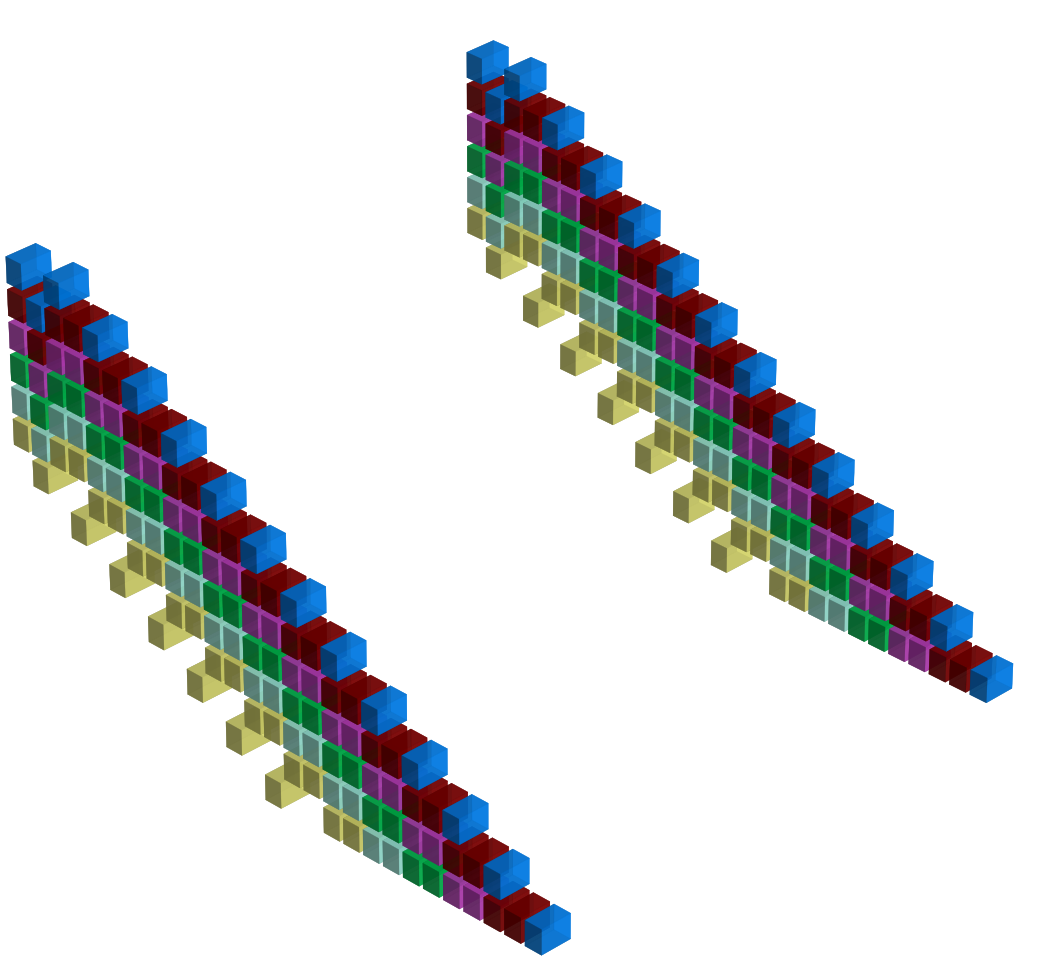
\includegraphics[width=3.2cm]{linemode/symmetries/pattern1-0-45.png}%
    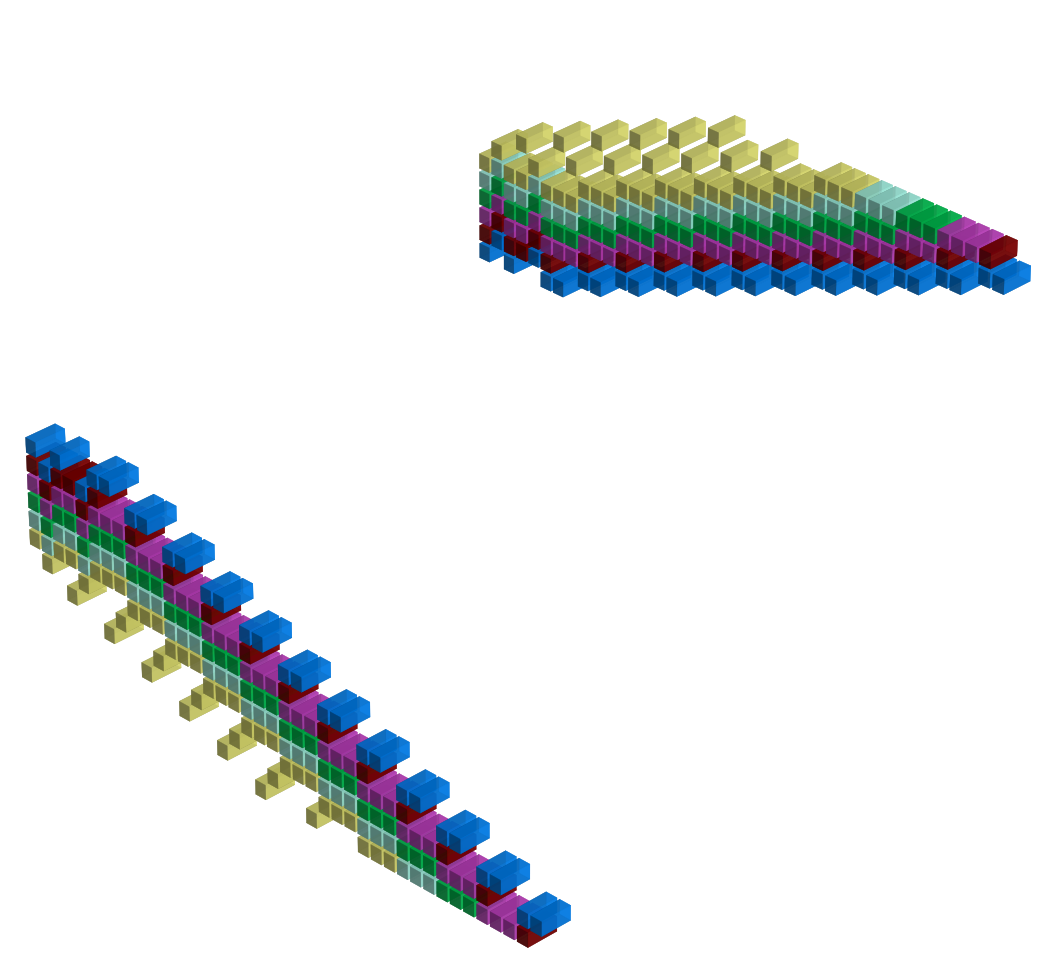
\includegraphics[width=3.2cm]{linemode/symmetries/pattern1-1-45.png}%
    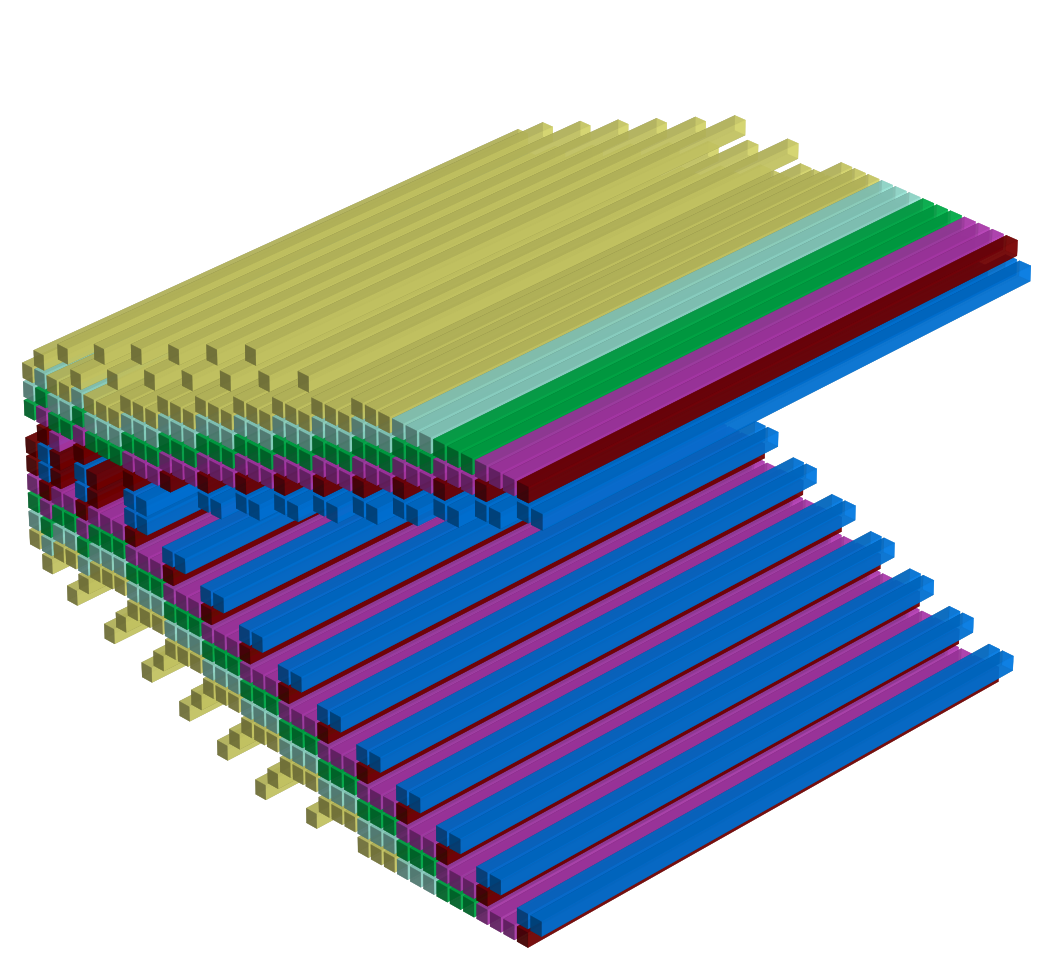
\includegraphics[width=3.2cm]{linemode/symmetries/pattern1-3-45.png}%
    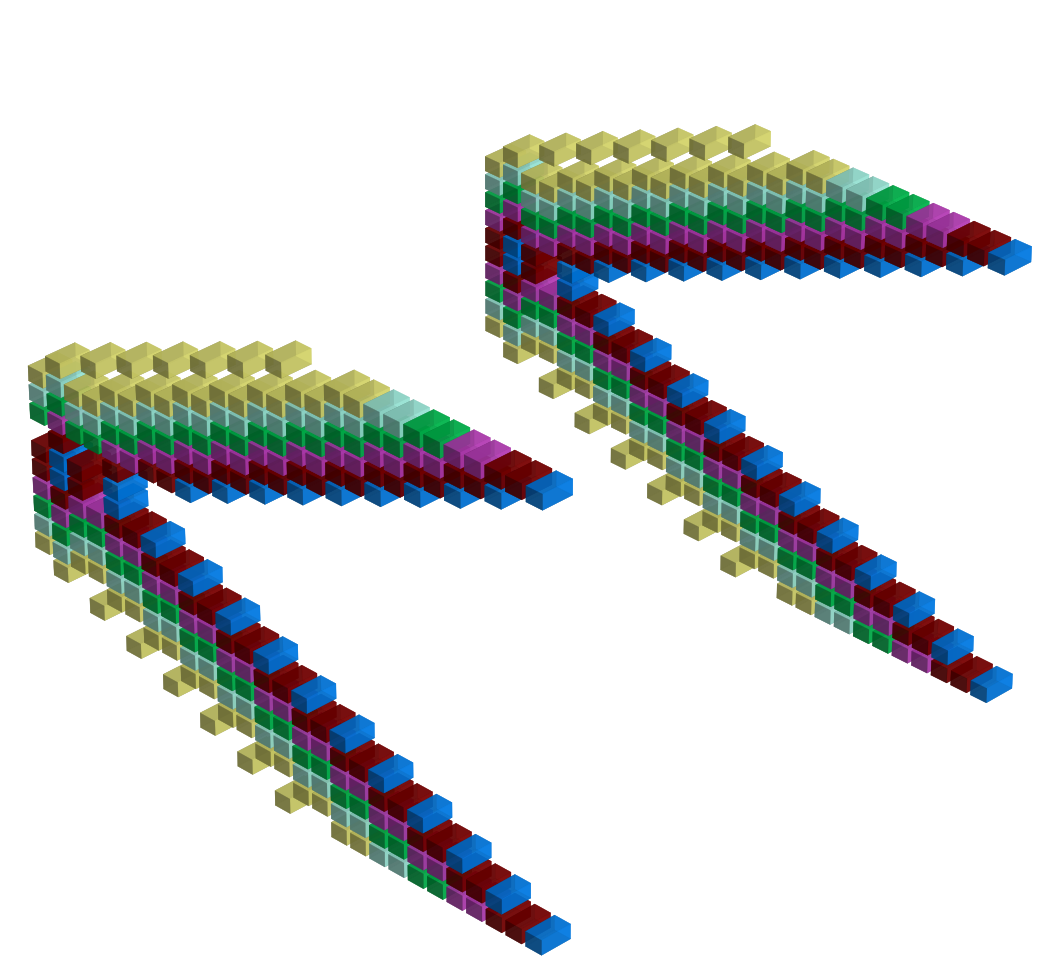
\includegraphics[width=3.2cm]{linemode/symmetries/pattern1-5-45.png}%
    \hspace{0.2cm}
    \caption{
      The different symmetries of Line Mode. 
      }
\end{figure}


\clearpage
